\documentclass{beamer}

\def\Tiny{\fontsize{6pt}{6pt}\selectfont}
\def\supertiny{\fontsize{4pt}{4pt}\selectfont}

\mode<presentation>
{
  \usetheme{Warsaw}
  % \setbeamercovered{transparent}
  \usecolortheme{crane}
}


\usepackage{graphicx, ifthen, listings}

\usepackage[czech]{babel}
% \usefonttheme{professionalfonts}
\usepackage{times}
\usepackage{amsmath}
\usepackage[utf8]{inputenc}
\usepackage{wrapfig}

\usepackage[T1]{fontenc}

\lstset{ basicstyle=\tiny, stringstyle=\ttfamily, showstringspaces=false }

\everymath{\displaystyle}

\setbeamerfont{frametitle}{size=\large}
\setbeamerfont{subsection in toc}{size=\scriptsize}

\makeatletter\newenvironment{blackbox}{%
   \begin{lrbox}{\@tempboxa}\begin{minipage}{0.95\columnwidth}}{\end{minipage}\end{lrbox}%
   \colorbox{black}{\usebox{\@tempboxa}}
}\makeatother

\title[IMF (2)]{Informatika pro moderní fyziky (2)\\základy Ruby, zpracování textu}

\author[Franti\v{s}ek HAVL\r{U}J, ORF ÚJV Řež]{Franti\v{s}ek HAVL\r{U}J\\{\scriptsize \emph{e-mail: haf@ujv.cz}}}

\date{akademický rok 2020/2021\\12. října 2020}

\institute[ORF ÚJV Řež]
{ÚJV Řež\\oddělení Reaktorové fyziky a podpory palivového cyklu}

\AtBeginSection[]
{
\begin{frame}<beamer>
\frametitle{Obsah}
\tableofcontents[currentsection,hideothersubsections]
\end{frame}
}

\begin{document}

\begin{frame}
  \titlepage
\end{frame}

\begin{frame}
  \tableofcontents
\end{frame}

\section{Co jsme se naučili minule}

\begin{frame}{}
  \begin{itemize}
    \item základní principy automatizace
    \item CSV soubory a Gnuplot
    \item příkazový řádek / terminál
    \item dávkové (BAT) soubory
    \item představení skriptovacích jazyků
    \item interpret Ruby a IRb
    \item letem světem Ruby
  \end{itemize}
\end{frame}


\section{Úvod do jazyka Ruby}

\subsection{Vstup a výstup}

\begin{frame}[fragile]{Výpis na terminál}
  \begin{block}{Print vs puts}
    \begin{verbatim}
      print "jedna"
      puts "dve"
    \end{verbatim}
  \end{block}
  \pause
  \begin{block}{Na všechno platí inspect}
    \begin{verbatim}
      puts "2 + 2 = #{2+2}"
      puts [1,2,3].inspect
    \end{verbatim}
  \end{block}
\end{frame}

\begin{frame}[fragile]{Iterátory}
  \begin{block}{Jednoduchý rozsah}
    \begin{verbatim}
      (1..5).each do
        puts "Cislo"
      end
    \end{verbatim}
  \end{block}
  \pause
  \begin{block}{S polem a proměnnou}
    \begin{verbatim}
      [1, 2, 3].each do |i|
        puts "Cislo #{i}"
      end
    \end{verbatim}
  \end{block}
\end{frame}

\begin{frame}[fragile]{Ještě jedna věc: formátovaný výstup}
  \begin{itemize}
    \item často potřebuju něco vytisknout `hezky', zarovnané, se správným počtem desetinných míst apod.
    \item v C na to je funkce \texttt{sprintf} a alternativa v Ruby funguje podobně
    \item je na to operátor \texttt{\%}: \emph{formát} \texttt{\%} \emph{data}
  \end{itemize}
  {\small
  \begin{verbatim}
"%10s" % "kolo"
"%-6d" % a
"%8.3f +- %8.3f" % [b, db]
  \end{verbatim}
  }
\end{frame}

\begin{frame}{Úlohy}
  \begin{itemize}
    \item vypište malou násobilku (ale hezky)
    \item vypište prvních N členů Fibonacciho posloupnosti (1, 1, 2, 3, 5, 8 ...)
    \item vypište všechna prvočísla menší než N
  \end{itemize}
\end{frame}

\begin{frame}[fragile]{Úlohy}
  \begin{block}{Násobilka / řešení}
\begin{verbatim}
(1..10).each do |a|
  (1..10).each do |b|
    puts "#{b} * #{a} = #{a*b}"
  end
end
\end{verbatim}
  \end{block}
  \pause
  \begin{block}{Násobilka / hezké řešení}
\begin{verbatim}
(1..10).each do |a|
  (1..10).each do |b|
    puts "%2d * %2d = %3d" % [b, a, a * b]
  end
end
\end{verbatim}
  \end{block}
\end{frame}

\begin{frame}[fragile]{Úlohy}
  \begin{block}{Fibonacci / řešení} \footnotesize
\begin{verbatim}
a, b = 1, 1
20.times do
  puts a
  c = a + b
  a = b
  b = c
end
\end{verbatim}
  \end{block}
  \begin{block}{Fibonacci / jiné řešení} \footnotesize
\begin{verbatim}
a, b = 1, 1
20.times do
  puts a
  a, b = b, a + b
end
\end{verbatim}
  \end{block}
\end{frame}

\begin{frame}[fragile]{Úlohy}
  \begin{block}{Erathostenovo síto / řešení}
\begin{verbatim}
n = 100

ary = (2..n).to_a
ary.each do |x|
  y = x
  while y <= n
    y += x
    ary.delete(y)
  end
end

puts ary.inspect
\end{verbatim}
  \end{block}
\end{frame}

\begin{frame}[fragile]{Čtení ze souboru}
  \begin{block}{Šikovný iterátor po řádcích}
    \begin{verbatim}
      File.foreach("data.txt") do |line|
        ...
      end
    \end{verbatim}
  \end{block}
  \pause
  \begin{block}{Celý soubor najednou}
    \begin{verbatim}
      string = File.read("data.txt")
    \end{verbatim}
  \end{block}
\end{frame}

\begin{frame}[fragile]{V podmínce}
  \begin{block}{If nebo Unless}
    \scriptsize
    \begin{verbatim}
      if "velikost".include?("kost")
        puts "s kosti"
      end
      unless 7 > 8
        puts "poporadku"
      end
    \end{verbatim}
  \end{block}
  \pause
  \begin{block}{Přirozený jazyk}
    \scriptsize
    \begin{verbatim}
      puts "je tam!" if "podvodnik".include? "vodnik"
      puts "pocty" unless 2 + 2 == 5
      a = [1]
      a << a.last * 2 while a.size < 10
    \end{verbatim}
  \end{block}
\end{frame}

\begin{frame}{Úlohy}
  V souboru \texttt{data/text\_1.txt}:
  \begin{itemize}
    \item spočítejte všechny řádky
    \item spočítejte všechny řádky s výskytem slova kapr
    \item spočítejte počet výskytů slova kapr (po řádcích i v kuse)
  \end{itemize}
\end{frame}

\begin{frame}[fragile]{Úlohy}
  \begin{block}{Kapři / řešení}
    \tiny
\begin{verbatim}
  n, n_kapr, nn_kapr = 0, 0, 0
  File.foreach("../data/text_1.txt") do |line|
    n += 1
    n_kapr += 1 if line.include?("kapr")
    nn_kapr += line.scan("kapr").size
  end

  nn_kapr_bis = File.read("../data/text_1.txt").scan("kapr").size

  puts "Celkem radku: #{n}"
  puts "Radku s kaprem: #{n_kapr}"
  puts "Celkem kapru: #{nn_kapr}"
  puts "        nebo: #{nn_kapr_bis}"
\end{verbatim}
  \end{block}
\end{frame}

\begin{frame}[fragile]{Zápis do souboru}
  \begin{block}{Soubor se otevře a pak už to známe}
    \begin{verbatim}
      f = File.open("text.txt", 'w')
      f.puts "Nazdar!"
      f.close
    \end{verbatim}
  \end{block}
  \pause
  \begin{block}{The Ruby way}
    \begin{verbatim}
      File.open("text.txt", 'w') do |f|
        f.puts "Nazdar!"
      end
    \end{verbatim}
  \end{block}
\end{frame}

\begin{frame}{Úlohy}
  Z dat v souboru \texttt{data/data\_two\_1.csv}:
  \begin{itemize}
    \item vyberte pouze druhý sloupec
    \item sečtěte oba sloupce do jednoho
    \item vypočtěte součet obou sloupců
    \item vypočtěte průměr a RMS druhého sloupce
  \end{itemize}
  S hvězdičkou:
  \begin{itemize}
    \item použijte soubory \texttt{*multi*}
    \item proveďte pro všechny čtyři CSV soubory
  \end{itemize}
\end{frame}

\begin{frame}[fragile]{Úlohy}
  \begin{block}{CSV(1) / řešení}
    \scriptsize
\begin{verbatim}
  File.open("druhy_sloupec.csv", 'w') do |f|
    File.foreach("../data/data_two_1.csv") do |line|
      f.puts line.strip.split[1]
    end
  end
\end{verbatim}
  \end{block}
\end{frame}

\begin{frame}[fragile]{Úlohy}
  \begin{block}{CSV(2) / řešení}
    \scriptsize
\begin{verbatim}
  File.open("sectene_sloupce.csv", 'w') do |f|
    File.foreach("../data/data_two_1.csv") do |line|
      data = line.strip.split
      f.puts data[0].to_f + data[1].to_f
    end
  end
\end{verbatim}
  \end{block}
\end{frame}

\begin{frame}[fragile]{Úlohy}
  \begin{block}{CSV(3) / řešení}
    \scriptsize
\begin{verbatim}
  x0 = 0
  x1 = 0
  n = 0
  File.foreach("../data/data_two_1.csv") do |line|
    data = line.strip.split
    x0 += data[0].to_f
    x1 += data[1].to_f
    n += 1
  end
  puts "Prvni sloupec: soucet #{x0}"
  puts "Druhy sloupec: soucet #{x1}"
\end{verbatim}
  \end{block}
\end{frame}

\begin{frame}[fragile]{Úlohy}
  \begin{block}{CSV(4) / řešení}
    \scriptsize
\begin{verbatim}
...
a0 = x0 / n
a1 = x1 / n

rms0 = 0
rms1 = 1
File.foreach("../data/data_two_1.csv") do |line|
  data = line.strip.split
  rms0 += (data[0].to_f - a0) ** 2
  rms1 += (data[1].to_f - a1) ** 2
  n += 1
end
rms0 = (rms0 / n) ** 0.5
rms1 = (rms1 / n) ** 0.5
puts "Prvni sloupec: RMS #{rms0}"
puts "Druhy sloupec: RMS #{rms1}"
\end{verbatim}
  \end{block}
\end{frame}


\subsection{Problém č. 2: jehla v kupce sena}

\begin{frame}{Zadání}
  \begin{block}{\# 2}
    Adresář plný CSV souborů (stovky souborů) obsahuje data, která jsou záznamy signálů s lineární závislostí.

    V pěti z nich jsou ale poruchy - data ležící zcela mimo přímku.

    Kde?
  \end{block}
\end{frame}

\begin{frame}{Příklad - dobrý signál}
  \begin{center}
      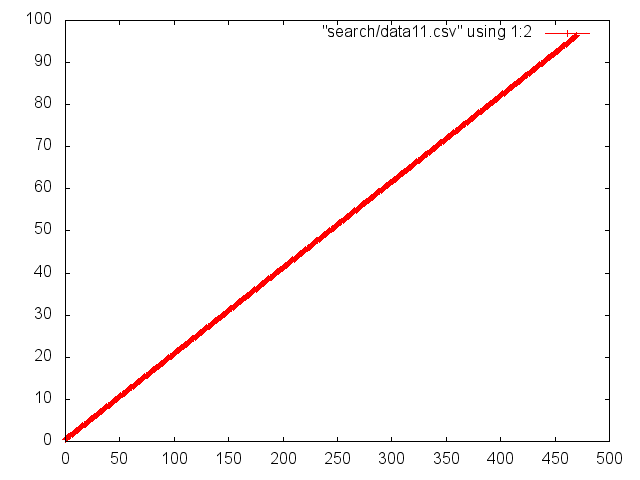
\includegraphics[width=0.6\columnwidth]{search_good}
      \end{center}
\end{frame}
\begin{frame}{Příklad - špatný signál}
  \begin{center}
      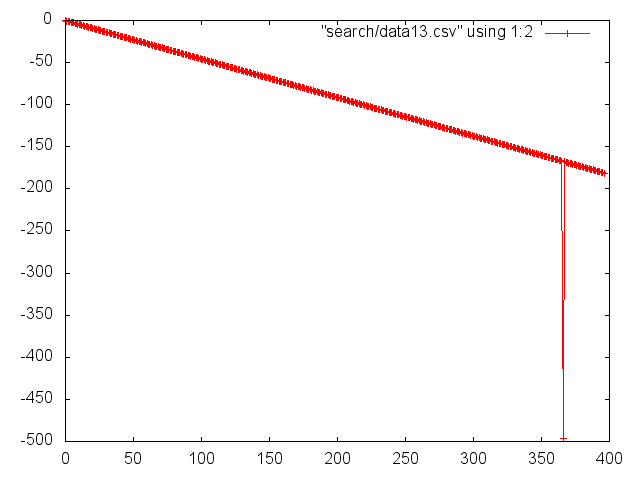
\includegraphics[width=0.6\columnwidth]{search_bad}
      \end{center}
\end{frame}

\begin{frame}{Řešení}
  \begin{itemize}
    \item stačí vykreslit grafy pro všechny
    \item \texttt{Dir} pro najití souborů
    \item připravit a spustit \texttt{gnuplot}
  \end{itemize}
\end{frame}

\begin{frame}{Znovu a lépe}
  \begin{itemize}
    \item pořád je to ještě spousta práce; navíc co když bude souborů tisíckrát víc?
    \item nabízí se několik řešení, od těžkopádných a robustních (LLS) přes chytré (selská regrese) až po jednoduché (detekce delta-y)
    \item hurá do toho, už je to jenom práce a skvělé cvičení
  \end{itemize}
\end{frame}

\section{Rozšíření Ruby: RubyGems a Bundler}

\begin{frame}{Knihovny (gemy) jsou základ}
  \begin{itemize}
    \item existují mnohá rozšíření, tzv. knihovny -- v ruby se jim říká rubygems
    \item aktuálně nás zajímá něco na práci s excelovskými soubory
    \item gemy jdou sice instalovat na systémové úrovni, ale z toho je pak zase jenom neštěstí
    \item použijeme radši \textbf{bundler}, správce gemů pro každého: vyřeší za nás závislosti a postará se o snadnou instalaci
  \end{itemize}
\end{frame}

\begin{frame}{Máme bundler?}
  \begin{itemize}
    \item otestujeme rubygems: \texttt{gem -v}
    \item pokud není, zapláčeme, protože jsme asi špatně nainstalovali Ruby
    \item otestume bundler: \texttt{bundle -v}
    \item pokud bundler není, doinstalujeme \texttt{gem install bundler}
  \end{itemize}
\end{frame}

\begin{frame}{Jak na to}
  \begin{itemize}
    \item najdu si, která knihovna mě zajímá (třeba na rubygems.org nebo kdekoli jinde): my bychom rádi rubyXL \texttt{https://github.com/weshatheleopard/rubyXL}
    \item vytvořím si prázdný \texttt{Gemfile} -- tam se specifikuje, které gemy chci používat: \texttt{bundle init}
    \item do gemfilu -- je to normální Ruby skript! -- dopíšu \texttt{gem "rubyXL"}
    \item nainstaluju: \texttt{bundle install --path vendor/bundle} (ten parametr stačí poprvé, bundler si to pak pamatuje v konfiguráku \texttt{bundle/.config})
  \end{itemize}
\end{frame}

\begin{frame}{Jak použít?}
  \begin{itemize}
    \item na začátku svého skriptu pak musím nahrát bundler:
    \item \texttt{require "bundler/setup"}
    \item a teď už můžu nahrát jakýkoli gem:
    \item \texttt{require "rubyXL"}
  \end{itemize}
\end{frame}

\section{Vytvoříme excelovskou tabulku}

\begin{frame}[fragile]{RTFM, RTFM, RTFM}
  \begin{itemize}
    \item na stránkách \texttt{rubyXL} se nachází spousta příkladů a návodů -- https://github.com/weshatheleopard/rubyXL
    \item kromě toho má i slušnou dokumentaci (GIYF / "rubyxl docs") -- http://www.rubydoc.info/gems/rubyXL/3.3.15
    \item naoprvé navedu do začátku:
  \end{itemize}
  {\tiny
  \begin{verbatim}
    workbook = RubyXL::Workbook.new
    worksheet = workbook[0]
    worksheet.add_cell(0, 0, 'A1')
    workbook.write("data.xlsx")
  \end{verbatim}
  }
\end{frame}

\begin{frame}{Jednoduché cvičení}
  \begin{itemize}
    \item použijte soubor \texttt{data\_two\_1.csv}
    \item vytvořte excelovský soubor se dvěma listy, na obou bude sloupec 1, sloupec 2 a součet
    \item na jednom součet bude jako číslo (sečte to váš skript)
    \item na druhém bude součet jako excelovský vzorec
  \end{itemize}
\end{frame}

\begin{frame}{A to je vše, přátelé!}
  \begin{center}
    
\includegraphics[width=0.8\textwidth]{looney_tunes}
  \end{center}
\end{frame}

\end{document}
